\subsection{Private Company Valuation}

\begin{figure}[H]
\centering
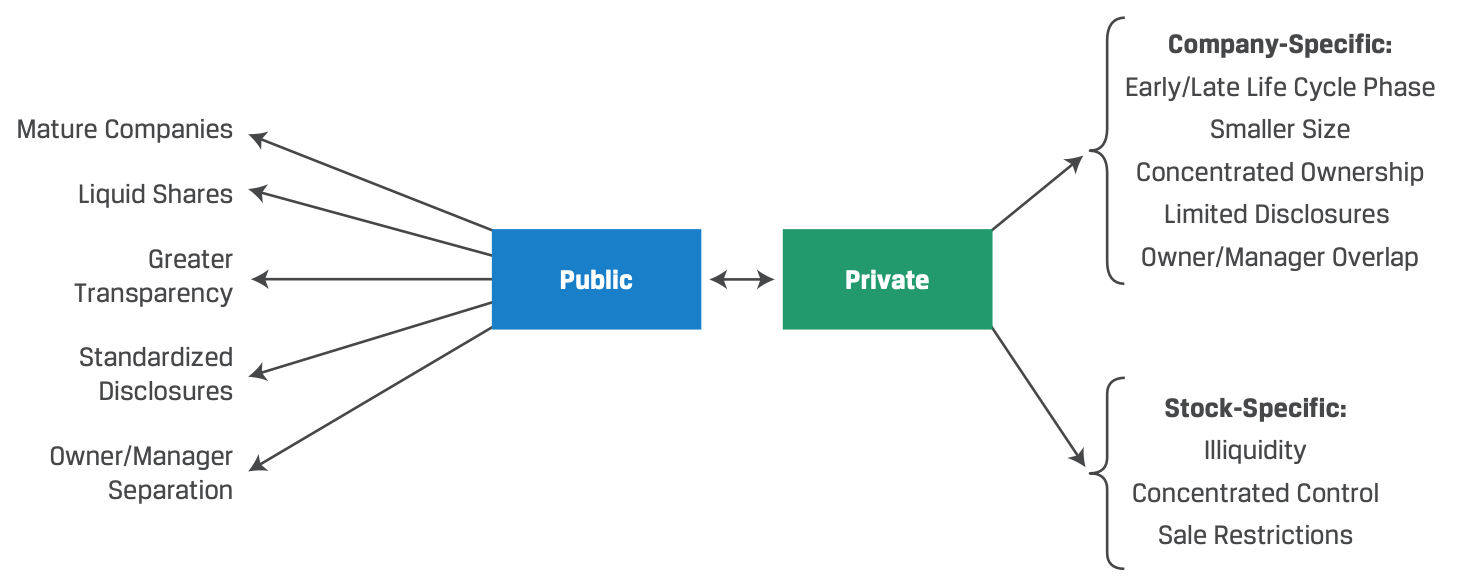
\includegraphics[scale=0.6]{/equity/pubvspriv}
\caption{Public vs Private Company Features}
\end{figure}

\begin{remark} \hlt{Company-Specific Features}
\begin{enumerate}[label=\roman*.]
\setlength{\itemsep}{0pt}
\item Stage of Life Cycle: private companies are typically less mature than public firms. In some circumstances, private companies are mature firms or bankrupt firms near liquidation. Valuation analysis vary with life cycle stage of the firm.
\item Size: Private firms typically. have less capital, fewer assets, fewer employees, hence are riskier. Thus private companies are valued using greater risk premiums and greater required returns. Lack of access to public equity markets may constrain private firm's growth, but regulatory burden associated with issuing public equity may outweigh benefit of greater access to funds.
\item Quality and Depth of Management: smaller private firms may not be able to attract as many qualified applicants as public firms, hence reducing the dept of management, slow growth and increasing risk.
\item Manager/Owner Overlap: in most private firms, management has substantial ownership position, reducing principal-agent conflict. External shareholders have little influence, allowing for longer-term perspectives.
\item Short-Term Investors: management in public firms take shorter-term view as compared to private firms where managers are long-term holders of significant equity interests.
\item Quality of Financial and Other Information: investor or creditor in a private firm will have less information than available for a public firm, leading to greater uncertainty, higher risk, reducing private firm valuation. Fairness opinions for private firm valuations relies on firm's financial statements and business records.
\item Taxes: private firms may be more concerned with taxes than public firms.
\end{enumerate}
\end{remark}

\begin{remark} \hlt{Stock-Specific Features}
\begin{enumerate}[label=\roman*.]
\setlength{\itemsep}{0pt}
\item Liquidity: private company equity has fewer potential owners and is less liquid than publicly traded equity. Hence a liquidity discount is often applied to valuing privately held shares.
\item Restrictions on Marketability: private companies have agreements to prevent shareholders from selling.
\item Concentration of Control: control of private firms is usually concentrated in hands of few shareholders, may lead to greater perks and other benefits to owners/managers at expense of minority shareholders.
\end{enumerate}
\end{remark}

\begin{remark} \hlt{Transaction-Related Valuations}
\begin{enumerate}[label=\roman*.]
\setlength{\itemsep}{0pt}
\item Venture Capital Financing: early-stage or VC firms see equity investors through multiple rounds of financing tied to achievement of key company developments or milestones. Less formal valuations are used as basis for negotiation between company and prospective investors
\item Private Equity Financing: growth or buyout transactions. Growth equity funds take minority stake in companies that has potential for scalable and renewed growth, with goal of exiting at higher valuation. Leveraged buyout funds acquire majority control to create value with more efficient business and optimising the balance sheet
\item Debt Financing: lenders perform valuation as part of underwriting process
\item Initial Public Offering: investment banks perform valuation using values of similar firms as a benchmark
\item Acquisitions and Divestitures: purchase or sale of stand-alone company or existing company division or line of business is common strategy for development-stage or mature companies.
\item Bankruptcy: to determine if a company is more valuable as a going concern or in liquidation. For viable concerns operating in bankruptcy, used for restructuring of over-leveraged capital structure.
\item Share-Based Incentive Compensation: stock option grants will require frequent valuations
\end{enumerate}
\end{remark}

\begin{remark} \hlt{Compliance-Related Valuations}
\begin{enumerate}[label=\roman*.]
\setlength{\itemsep}{0pt}
\item Financial Reporting: related to goodwill impairment tests, where units of a public firm are valued using private company valuation methods. Reporting of stock-based compensation also requires these methods.
\item Tax Purposes: at firm level, transfer pricing, property taxes, and corporate restructuring may necessitate valuations. For individual equity owners, estate and gift tax issues may necessitate valuations.
\item Litigation: for shareholder suits, damage claims, lost profit insurance claims, or divorce settlements.
\end{enumerate}
\end{remark}

\begin{figure}[H]
\centering
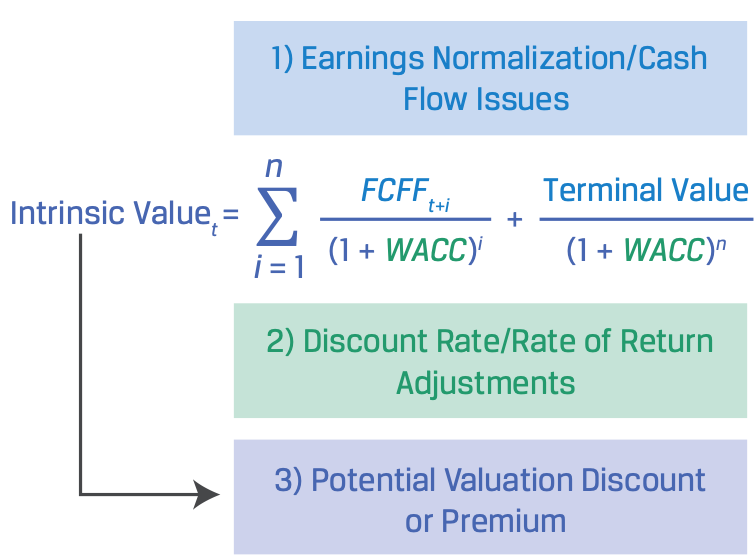
\includegraphics[scale=0.5]{/equity/pcval}
\caption{Private company valuation considerations}
\end{figure}

\subsubsection{Earnings Normalisation and Cash Flow Estimation}

\begin{figure}[H]
\centering
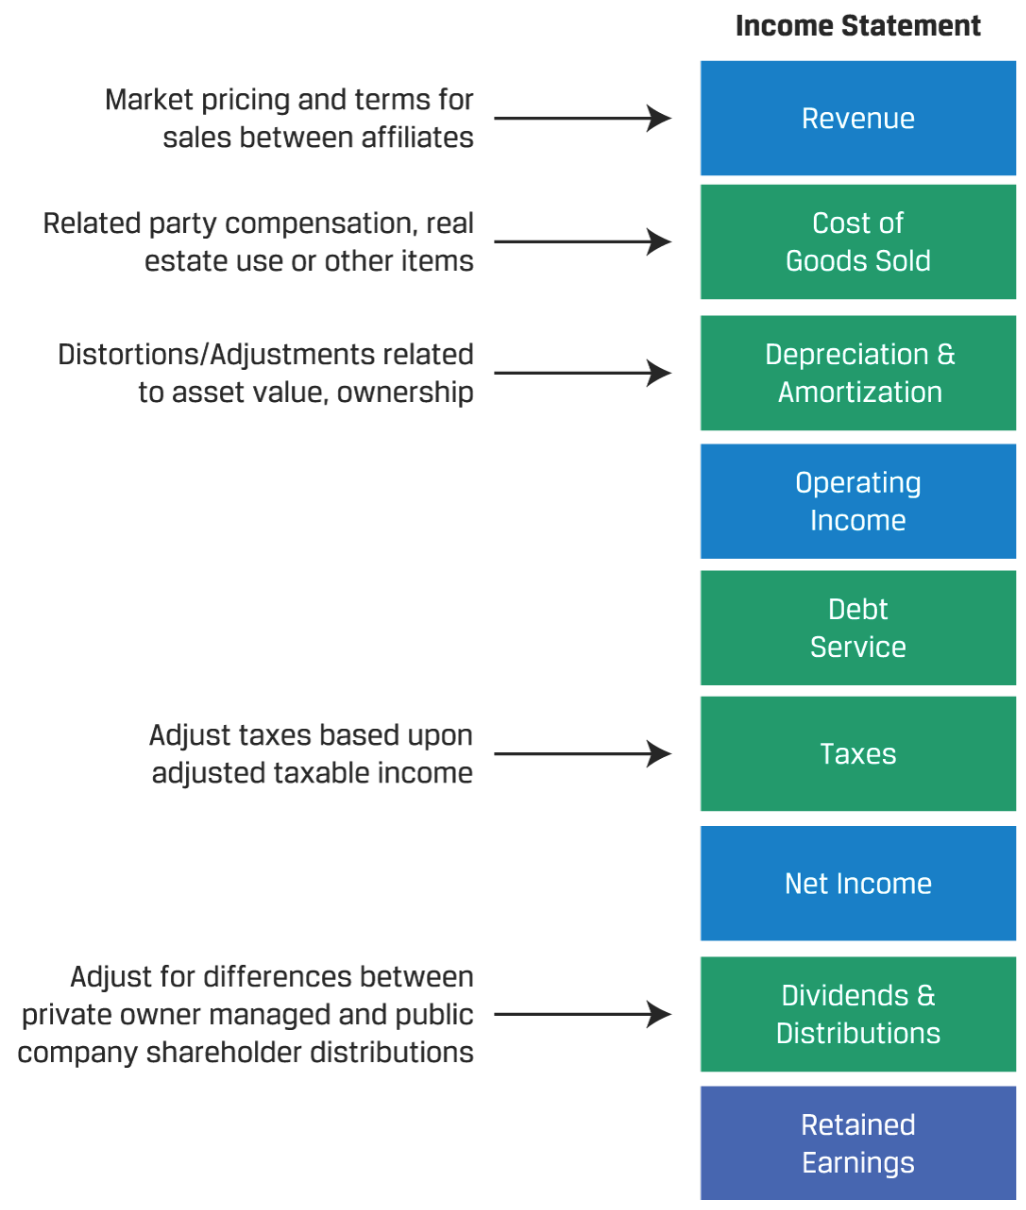
\includegraphics[scale=0.5]{/equity/pcisadj}
\caption{Private company selected earnings adjustments}
\end{figure}

\begin{remark} \hlt{Earnings Normalisation Issues}\\
Normalised earnings should exclude non-recurring, non-economic, unusual items. Private firms with concentrated control may have discretionary or tax-motivated expenses that need to be adjusted.
\begin{enumerate}[label=\roman*.]
\setlength{\itemsep}{0pt}
\item Closely controlled firm may conduct business with its owners or other businesses controlled by its owners, and inflating firm expenses. Artificially low earnings may be a result of excessively high owner compensation, or personal expenses charged to the firm. Use of company-owned assets may require adjustments.\\
If firm is performing poorly, owners may be receiving compensation below market levels, and hence reported earnings would overstate normalised earnings.
\item Real estate owned by firm may require separate treatment from firm operations, as it may have different risk characteristics from firm's operations.\\
Properties depreciation expense is based on historical cost and does not reflect current rental cost.\\
To remove any income and expenses from real estate on income statement. If it is used in firm's business, market-estimated rental expense is used in estimating earnings.\\
Value of real estate is hence separated from operations and treated as non-operating asset.\\
If real estate is leased from related party, lease rate should be adjusted to market rate.
\item Some private firm financial statements are reviewed rather than audited, some may only be compiled.
\item Other adjustments are common to both private and public companies, i.e., adjustment for differences in depreciation and inventory methods.
\end{enumerate}
\end{remark}

\begin{remark} \hlt{Cash Flow Estimation Issues}\\
The equity interest appraised and intended use of appraisal is key in determining appropriate definition of value for a specific valuation.
\begin{enumerate}[label=\roman*.]
\setlength{\itemsep}{0pt}
\item If there is significant uncertainty on private company's future operations, to examine several scenarios when estimating future cash flows. For companies in development, scenarios include IPO, acquisition, continued private operation, or bankruptcy. For mature firm, scenarios include a range of cash flows based on different assumed growth rates.\\
For each scenario, to assign a discount rate and probability based on the scenario's risk and probability of occurring. Firm value is estimated for each scenario, and a weighted average of these values is the estimated firm value; alternatively, a weighted average scenario cash flow may be discounted at a single discount rate to arrive at a firm value.
\item Cash flow estimates to be based on current management estimates, or result from consultation with management. To be aware of potential bias in management estimates, as management may overstate value of goodwill or understate future capital needs.
\end{enumerate}
FCFF is more appropriate when significant changes in firm's capital structure is anticipated, as WACC is less sensitive to changes in leverage.
\end{remark}

\begin{remark} \hlt{Estimation of Discount Rate}
\begin{enumerate}[label=\roman*.]
\setlength{\itemsep}{0pt}
\item Size Premiums: added to discount rate for small private companies. Estimate of premium is based on public data for smallest market cap segments, but may be biased upward as some of the small firms were formerly larger companies that are now in financial and/or operating distress.
\item Availability and Cost of Debt: private firm has less access to debt financing than a smaller public company, hence private firm may take on more equity financing, increasing its WACC. Smaller private firm may face greater operating risk and a higher cost of debt.
\item Acquisition Discount Rate: when larger companies acquire smaller companies, the buyer is expected to have lower cost of capital than target. Use of buyer's lower cost of debt from seller's perspective would imply buyer is paying seller for possible value it brings to a transaction due to its lower capital costs.
\item Projection Risk: lower availability of information on private firm may make it appropriate for analyst to apply higher discount rate. Private firm's management may be inexperienced at forecasting, making upward or downward adjustment of earnings forecast appropriate.
\item Life Cycle Stage: firms in early stage may have unusually higher levels of non-diversifiable risk, hence CAPM may be in appropriate. Although ranges of discount rates may be specified for various life cycle stages, it may be difficult to accurately classify the stage a firm is in.
\end{enumerate}
\end{remark}

\begin{method} \hlt{Adjusting Comparable Beta for Private Company}\\
First, un-lever the comparable public company beta using its tax rate and debt-to-equity ratio.
\begin{equation}
\beta_{\text{Unlevered}} = \frac{\beta_{\text{Public}}}{1 + (1-t)(\frac{D}{E})} \nonumber
\end{equation}
Adjust this un-levered beta using target private company's tax rate and leverage,
\begin{equation}
\beta_{\text{Private Company}} = \beta_{\text{Unlevered}}\left[1 + (1-t^*) \left(\frac{D}{E} \right)^* \right] \nonumber
\end{equation}
\end{method}

\begin{remark} \hlt{Alternatives to CAPM for Private Company Valuation}
\begin{enumerate}[label=\roman*.]
\setlength{\itemsep}{0pt}
\item Expanded CAPN: adds additional premium for small size and company-specific risk. Estimation of company-specific risk is subjective, conducted based on industry and company analysis, as well as comparable public companies (guideline public companies).
\item Build-Up Approach: used when comparable public companies are unavailable or of questionable comparability. Approach begins with expected return on market (beta implicitly assumed to be one), premiums added for small size, industry factors, company-specific factors.
\end{enumerate}
\end{remark}

\begin{figure}[H]
\centering
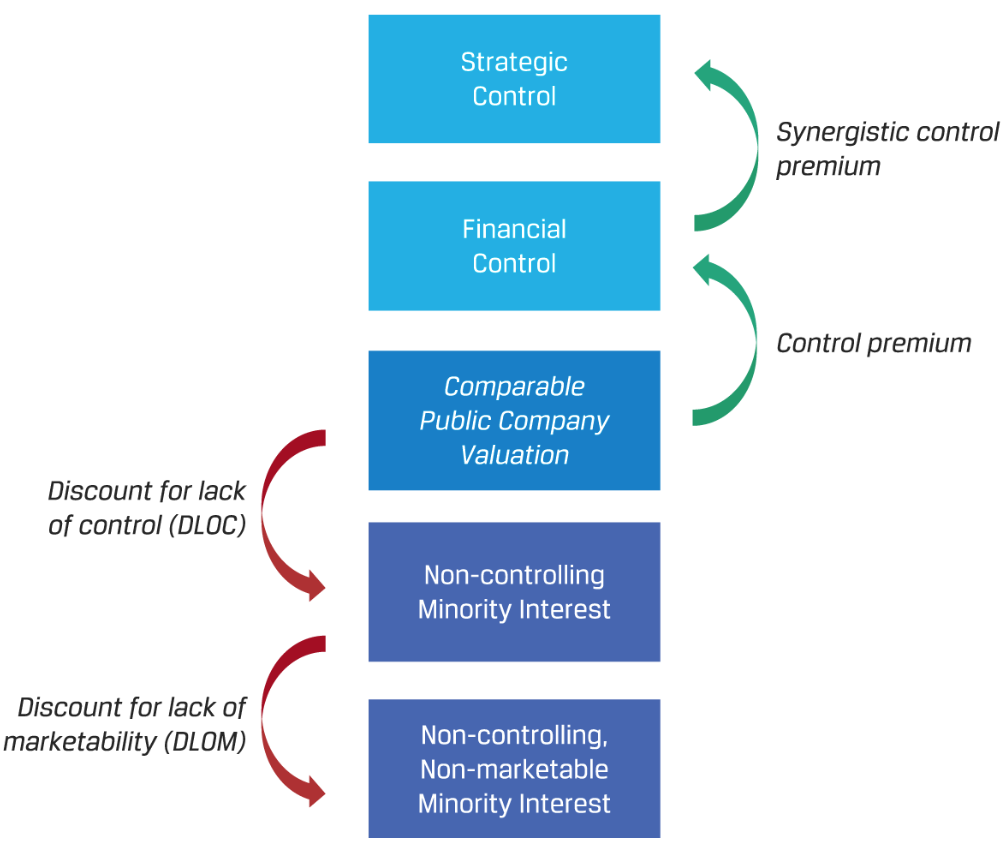
\includegraphics[scale=0.5]{/equity/pcdisprem}
\caption{Private company valuation discounts and premiums}
\end{figure}

\begin{remark} \hlt{Valuation Discounts and Premiums}
\begin{enumerate}[label=\roman*.]
\setlength{\itemsep}{0pt}
\item Strategic Buyer: valuation based on perceived synergies with acquirer's other assets. Buyer is also willing to assume the execution risk associated with their realisation.
\item Financial Buyer: buyer unable to identify synergies, may be unable or unwilling to take advantage of them due to lack of operational or management expertise, or has limited risk appetite.
\item Discount for Lack of Control (DLOC): minority shareholders have less power to select directors and management than controlling shareholders, and cannot determine the investment policies and payout policies that will affect the value of the firm and distribution of earnings. \\
Estimates of DLOC is estimated using control premium data from public company acquisitions.
\begin{equation}
\text{DLOC} = 1 - \left[\frac{1}{1 + \text{Control Premium}} \right] \nonumber
\end{equation}
Valuations based on DCF methods could also require adjustments, depending on whether the estimated and subject CF were on a controlling or non-controlling interest basis.
\item Discount for Lack of Marketability (DLOM): used when interest in a firm cannot be easily sold. Impending IPO or firm sale, and larger pool of buyers will decease DLOM. Contractual restrictions on selling stock and greater ownership concentration will increase DLOM. Methods for estimating DLOM are as follows:
\begin{enumerate}[label=\arabic*.]
\setlength{\itemsep}{0pt}
\item Price of restricted shares compared to price of publicly traded shares. Private sale of block of restricted shares may reflect valuation discount.
\item Price of pre-IPO shares compared to price of post-IPO shares. However, post-IPO firms generally have more certain CF and lower risk, hence DLOM estimated may not be pure.
\item Estimated as value of an at-the-money put option of a comparable public company, divided by its stock price. Time to maturity of the option should correspond to the time to IPO, volatility based on historical volatility of publicly trade stock, or implied volatility of publicly traded options.\\
Estimated risk of the private company can be factored into the option price, but a put option indicates a certain selling price, not actual liquidity.
\end{enumerate}
\end{enumerate}
If both DLOC and DLOM are applied, the total discount is as follows:
\begin{equation}
\text{Total Discount} = 1 - \left[(1-\text{DLOC})(1-\text{DLOM})\right] \nonumber
\end{equation}
In addition, other discounts such as key person discount, portfolio concentration discount, lack of voting rights discount may also apply.
\end{remark}

\subsubsection{Valuation Approaches}

\begin{remark} \hlt{Selection of Appropriate Valuation Approach}\\
Early life cycle firms is better valued using asset-based approach. As firm moves to high growth phase, income approach is more appropriate. A mature firm is most appropriately valued with market approach.\\
Price multiples from large public firms should not be used to value small private firms without assurance that risk and growth prospects of the firms are similar.\\
Valuation based on income or earnings multiples would not attach a value to non-operating assets. If these assets are significant portion of firm value, to be separately added when valuing a firm.
\end{remark}

\begin{figure}[H]
\centering
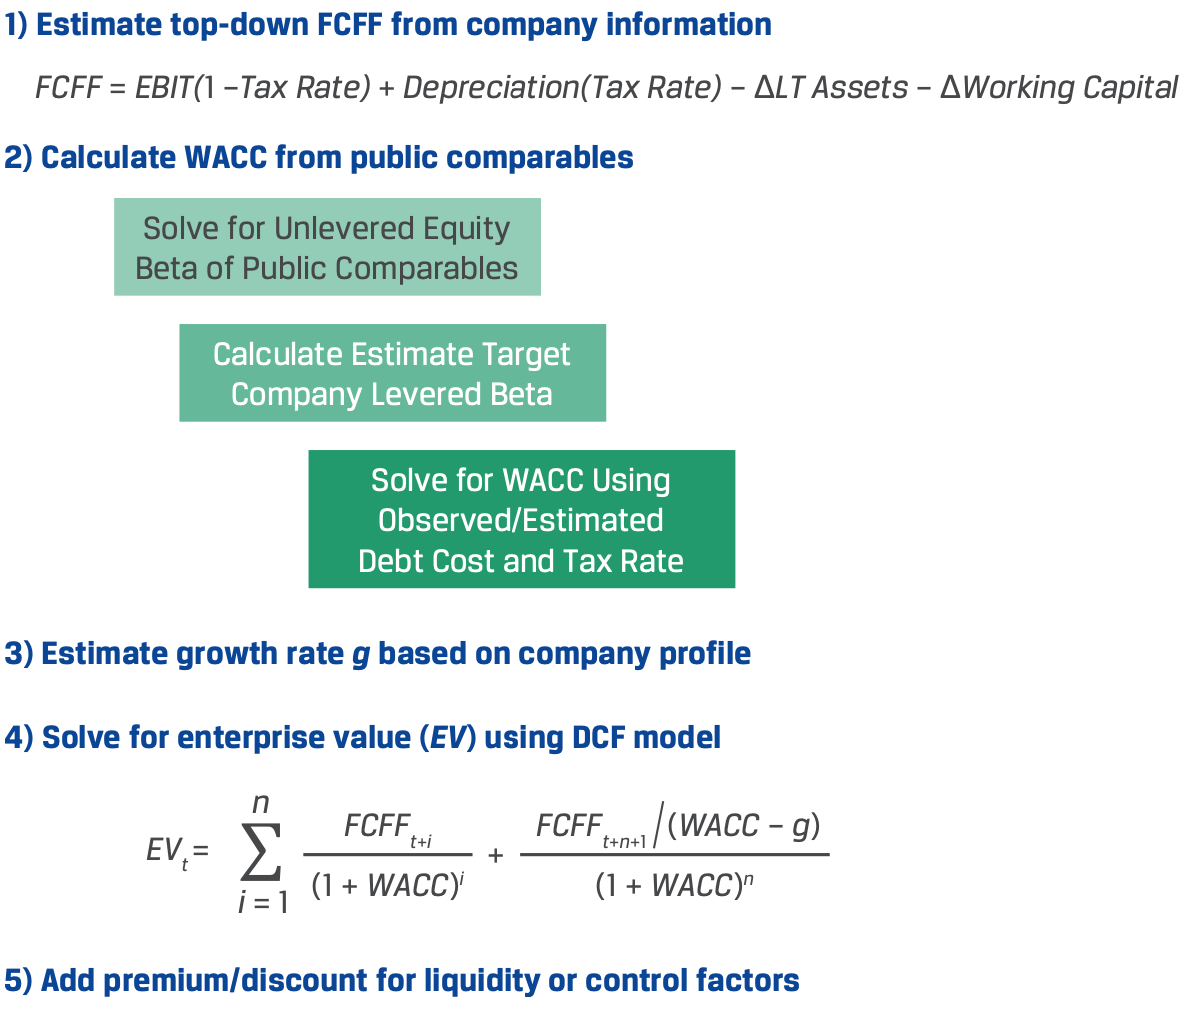
\includegraphics[scale=0.6]{/equity/incomeapp}
\caption{Private company income approach}
\end{figure}

\begin{method} \hlt{Income Approach: Free Cash Flow Method}\\
Series of discrete cash flows forecasted. Terminal year is when growth expected to level off and remain constant. Terminal value calculated with constant growth model (i.e., DDM), price multiple approach, or capitalised CF.\\
If price multiple is used for firm in high growth industry, the price multiple applied will reflect both high growth and normal growth; high growth will be double counted, once in price multiple and once in periodic CF forecasts.
\begin{equation}
\text{Intrinsic Value}_t = \sum\limits_{i=1}^n \frac{\text{FCFF}_{t+i}}{(1+\text{WACC})^i} + \frac{\text{Terminal Value}}{(1 + \text{WACC})^n} \nonumber
\end{equation}
\end{method}

\begin{figure}[H]
\centering
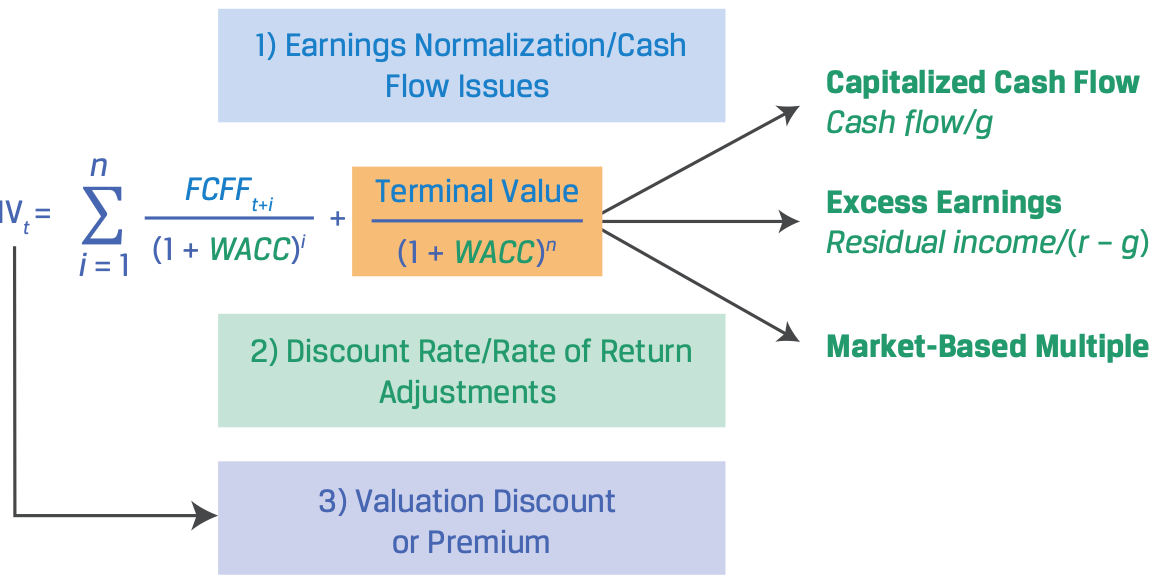
\includegraphics[scale=0.5]{/equity/pctva}
\caption{Private company terminal value approaches}
\end{figure}

\begin{method} \hlt{Income Approach: Capitalised Cash Flow Method (CCM)}\\
Estimates value based on company's projected performance as a growing perpetuity under stable growth.\\
Appropriate for private companies where no projections are available and/or market pricing evidence from similar public companies or transactions is limited.
\begin{equation}
\text{Firm Value}_t = \frac{\text{FCFF}_{t+1}}{\text{WACC} - g} \nonumber
\end{equation}
Expected FCFF may be estimated using firm's expected after-tax EBIT and reinvestment rate (b).
\begin{equation}
\text{b} = \frac{g}{\text{WACC}} \nonumber
\end{equation} 
Using projected EBIT, the firm value is then
\begin{equation}
\text{Firm Value}_t = \frac{\text{EBIT}_{t+1}(1-t)(1-b)}{\text{WACC}-g} \nonumber
\end{equation}
To get firm's intrinsic equity value (IV$_{t}$), subtract estimated market value of debt from firm's value. Use of constant WACC assumes capital structure will remain unchanged.\\
Market value of debt based no public debt on debt type, tenor, credit quality, industry etc.
\begin{equation}
\text{IV}_t = \frac{\text{FCFE}_{t+1}}{r_e - g} = \frac{\text{FCFE}_{t+1}}{\text{Capitalisation Rate}} \nonumber
\end{equation}
\end{method}

\begin{method} \hlt{Income Approach: Excess Earnings Method (EEM)}\\
Earnings estimated after deducting amounts that reflect required returns to working capital and fixed assets.
\begin{enumerate}[label=\arabic*.]
\setlength{\itemsep}{0pt}
\item Estimate firm's normalised earnings
\item Determine fair market value of tangible assets, including working capital and fixed assets, and required rates of return. Working capital is lowest risk and most liquid, hence have lowest required rate of return ($r_{\text{WC}}$); fixed assets require higher rate of return ($r_{\text{FA}}$). Intangible assets has limited liquidity and high risk, hence have highest return ($r_{\text{IA}}$).
\item Deduct required return on tangible assets from normalised earnings to solve for excess returns.
\end{enumerate}
\begin{equation}
\text{Residual Income}_t = \text{Normalised Income} - (\text{Working Capital} \times r_{\text{WC}}) - (\text{Fixed Asses} \times r_{\text{FA}}) \nonumber
\end{equation}
The residual income is capitalised with similar growth perpetuity formula in CCM to solve for present value of intangible assets (RV$_r$), with $g$ as RI growth rate.
\begin{equation}
\text{RV}_t = \frac{\text{Residual Income}_t (1+g)}{r_{\text{RI}} - g} \nonumber
\end{equation}
Firm value is sum of value of tangible assets and residual value of excess earnings from intangible assets.\\
Used to value intangible assets, very small businesses when other market approach methods are not feasible.
\end{method}

\begin{figure}[H]
\centering
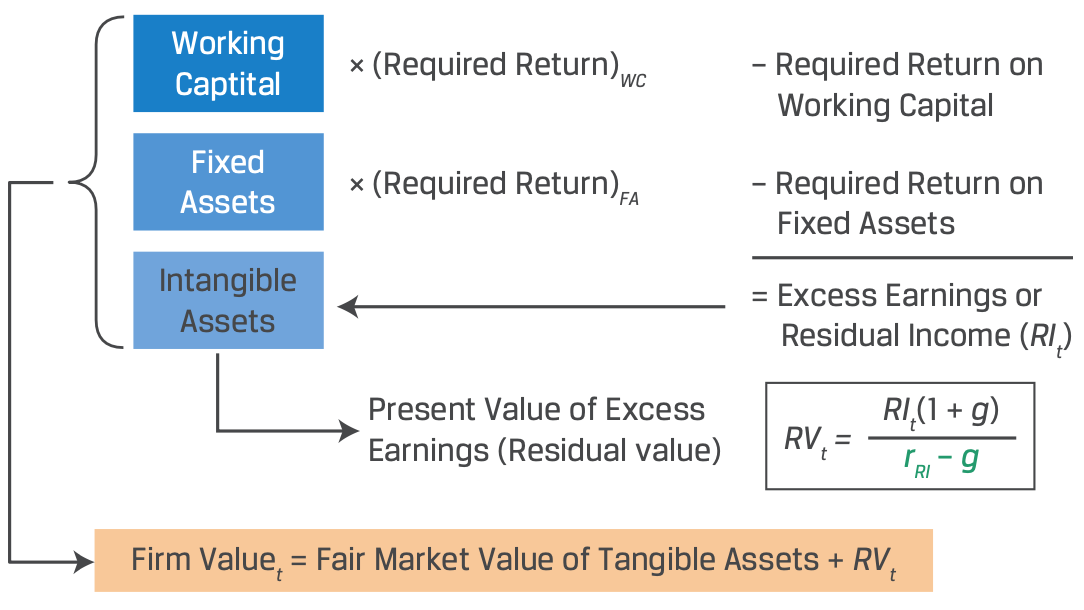
\includegraphics[scale=0.5]{/equity/pceem}
\caption{Private company excess earnings method}
\end{figure}

\begin{figure}[H]
\centering
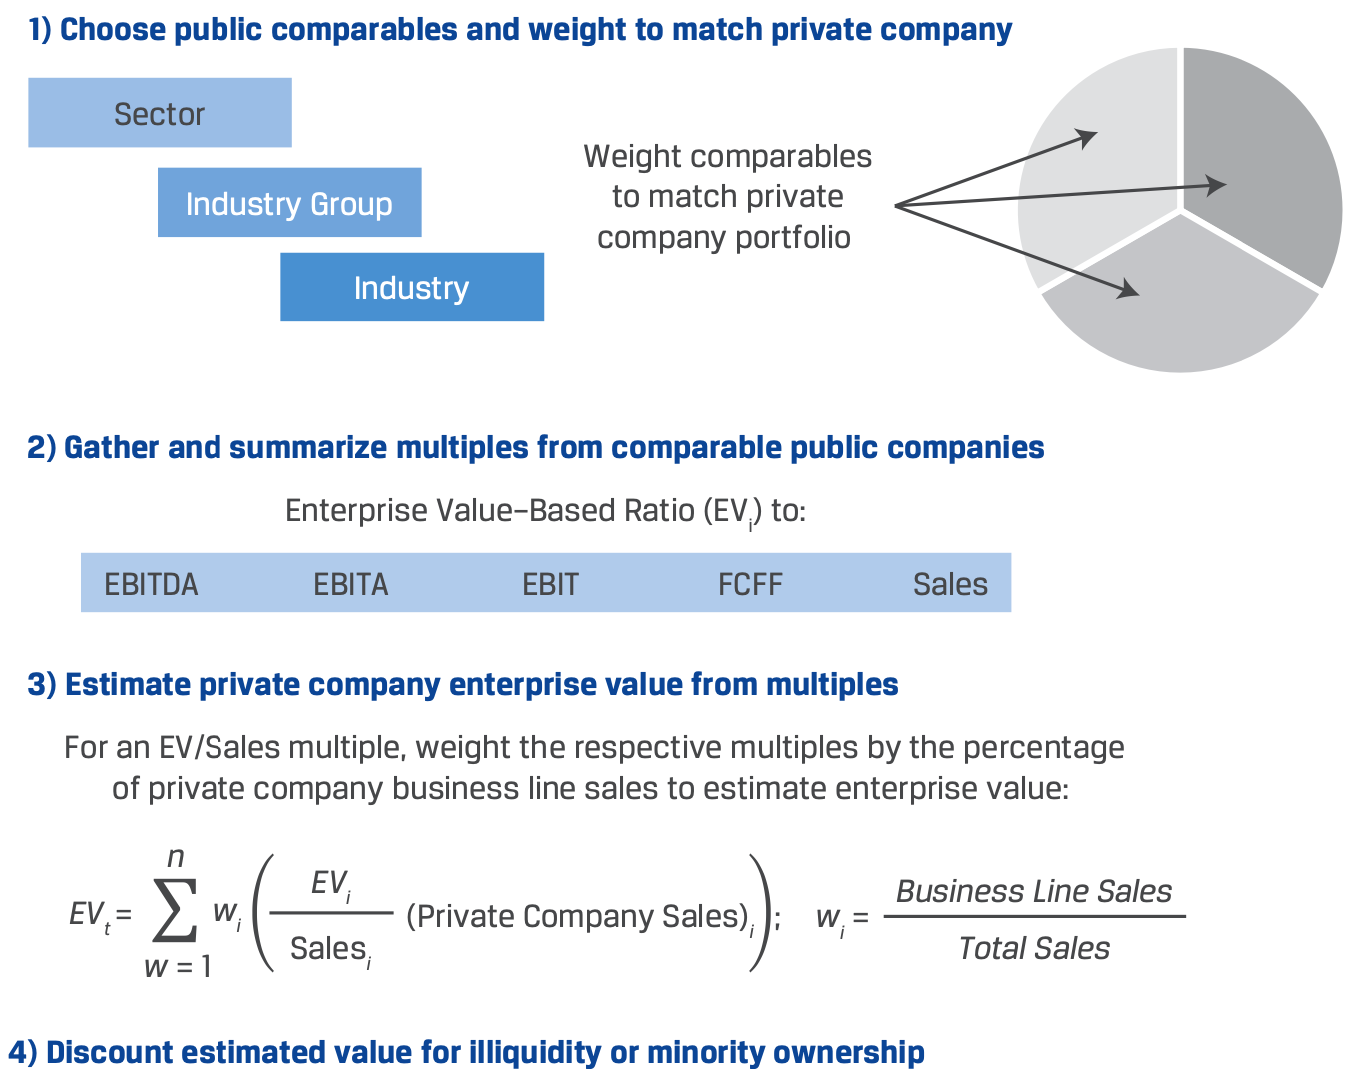
\includegraphics[scale=0.6]{/equity/mktapp}
\caption{Private company market-based approach}
\end{figure}

\begin{method} \hlt{Market-Based Approach: Guideline Public Company Method (GPCM)}\\
Enterprise value multiples from public companies are used, with adjustments to multiples to account for differences in size, leverage, and life cycle stage.\\
When evaluating a controlling equity interest in private firm, control premium should be estimated, which is the difference between pro rata value of controlling interest against that of non-controlling interest. Most public share trades are for small, non-controlling interests, hence price multiple do not reflect control premium.\\
To estimate control premium, the following issues should be considered:
\begin{enumerate}[label=\roman*.]
\setlength{\itemsep}{0pt}
\item Transaction Type: strategic or financial transaction may have different price premium
\item Industry Factors: industry sectors with active acquisition activity may already have control premium priced in the share prices. Control premiums measured at different time may reflect different industry environment from that of the valuation date.
\item Type of Consideration: estimates of control premium will be overstated when acquisitions are made with shares trading at inflated values.
\item Reasonableness: use of control premiums and price multiples may compound into significant deviations from historical pricing, which should be investigated.
\item Multiple Industries: private company operating in multiple industries to use a weighted average multiple based on proportion of revenues generated in each industry.
\item Other Factors: differences in size, country, tax status, leverage.
\end{enumerate}
\end{method}

\begin{method} \hlt{Market-Based Approach: Guideline Transactions and Prior Transaction Methods}\\
Prior acquisition values for entire companies are used, which already reflect control premiums, so no additional adjustment for controlling interest is necessary.\\
Issues to be considered are:
\begin{enumerate}[label=\roman*.]
\setlength{\itemsep}{0pt}
\item Transaction Type: strategic or financial transaction may have different price premium
\item Contingent Consideration: potential future payments to the seller contingent on achievement of certain milestones. As this increases the risk to the seller, transactions with contingent considerations to be scrutinised before comparison to transactions without such contingencies.
\item Non-Cash Consideration: acquisitions with large blocks of stock create uncertainty in transaction price.
\item Availability of transactions: meaningful transactions may be limited. Relevance of pricing indications from historical transaction to be challenged given significant changes in company, industry, economy.
\item Changes Between Transaction and Valuation Date: changes in market conditions may result in different risk and growth expectations, requiring in adjustment to the price multiple
\item Other factors; differences in company size, tax status, leverage
\end{enumerate}
\end{method}